\documentclass{scrartcl}

\usepackage{polyglossia,graphicx}
\setdefaultlanguage{swedish}

\begin{document}

\title{Project Scope}
\author{Group Joy}
\date{\today}
\maketitle

\section{Beskrivning}

Vi planerar att skapa en karta där användarna kan se data utspritt över de olika länen/regionerna och kommunerna i landet.
Datan som kommer att väljas kommer att begränsas till data som redan är indelad på kommunnivå och som är lätt tillgänglig för oss.
Kartan riktar sig mot alla sammhällsmedvetna medborgare i Sverige.

\subsection{Datakällor}

Vi kommer använda oss av kartor från OpenStreetMap projektet.
Statistiken kommer främst komma från SCB (Statistiska centralbyrån).

\subsection{beskrivande diagram av produkten}
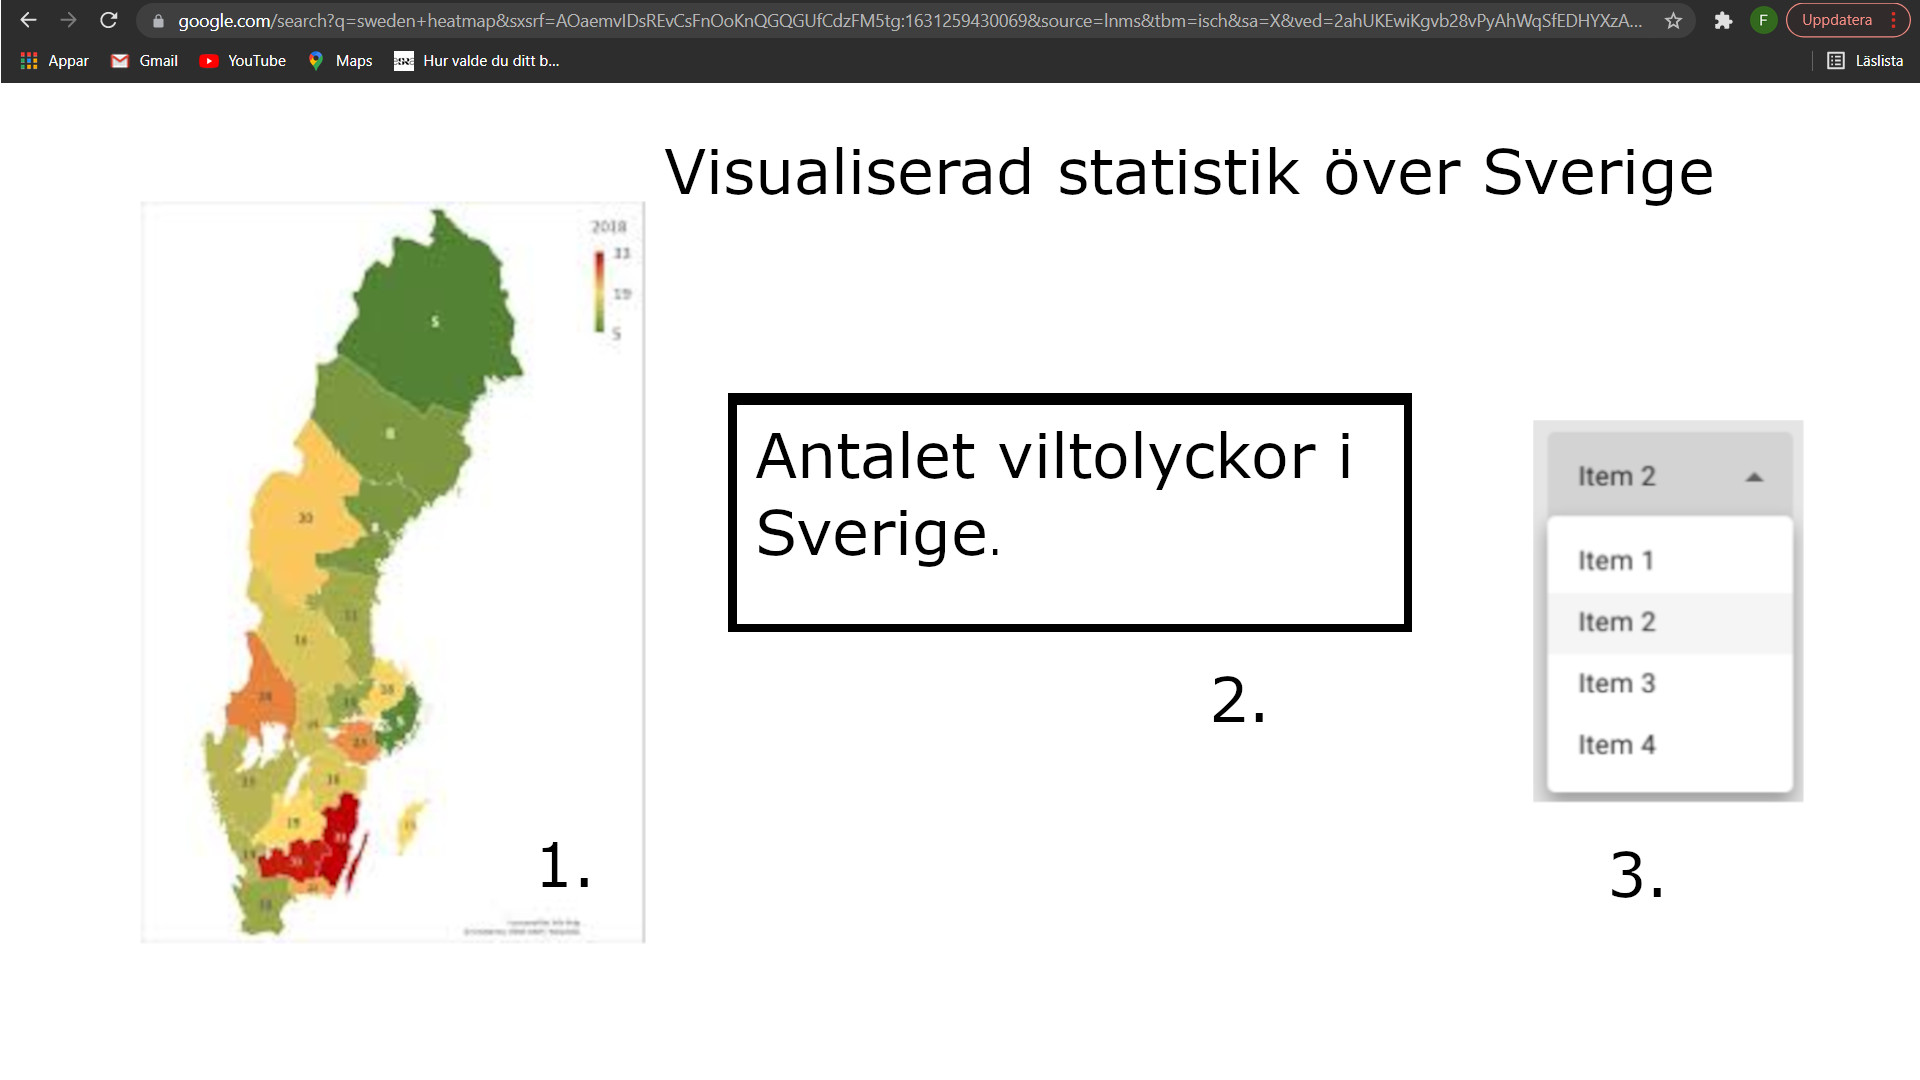
\includegraphics{dokument/mockup.jpg}

\begin{itemize}
\item 1. Heatmap som visar olika områden med olika färger baserat på vilka val som gjorts i menyn till höger. Det visas även en teckenförklaring/legend för vad  dem olika färgerna betyder.
\item 2. Kort information om statistiken som har valts, till exempel när statistiken är insamlad, vilka val som gjorts i menyn till höger etc. 
\item 3. Dropdown meny för att välja statistik att visa.
\end{itemize}

\section{Koppling till FNs hållbarhetsmål}

    Eftersom projektet är öppet och kommer bygga på så mycket olika data kommer projektet kunna kopplas till flera av FN's mål, och det är därför svårt att nu innan projektets början säga exakt vilka som kommer eller inte kommer kunna anknytas till projektet. Ett exempel är dock hållbara städer och samhällen, eftersom vi kan visa på befolkningstäthet, mängd avfall per region m.m.


\section{Affärsmodell}
\begin{itemize}
    \item \textbf{Värdeerbjudande} Vi skapar värde genom att förenkla visandet av data. Genom en heatmap kan användaren enkelt få en bild av vilka delar av landet som valt ämne påverkar mer eller mindre.
    \item \textbf{Kundsegment} En vardaglig användare är mer trolig att enkelt tolka data genom grafik istället för genom ren statistik, därav utökar vi demografin för uppvisande av statistik.
    \item \textbf{Nyckelaktiviteter} För att kunna leverera produkten kommer vi sätta upp större mål, och sedan bryta ner dem i mindre mål för att kunna uppnå dessa. Arbetssättet vi ska använda kallas scrum.
    \item \textbf{Nyckelresurser} SCBs olika öppna datakällor som vi kan använda oss av. Även kod bibliotek som förenklar utvecklingen av slutprodukten kommer vara en viktig del av arbetet.
\end{itemize}

\section{Teknik}

Vi planerar att applikationen kommer vara en webbapplikation där vi skriver back-enden i Python och front-enden i någon webbteknik.
Datan kommer att sparas i en SQL databas.

\end{document}